\begin{center}
\large Experimento: \textbf{Amplificador inversor e não inversor}
\end{center}


\section{Introdução}


O presente relatório visa detalhar o experimento laboratorial realizado na disciplina laboratório de circuitos eletrônicos no dia 10 de setembro de 2019 sobre amplificador inversor e não inversor utilizando amplificadores operacionais, mais especificamente os do circuito integrado LM741.

Esses amplificadores inversores e não inversores possuem as mais diversas aplicações. O que difere um do outro é que o primeiro inverter a fase do sinal em 180° e o segundo não, como o próprio nome sugere. As características do Amp Op de alta impedância de entrada, baixa impedância de saída e ganho de tensão estável tornam o amplificador com Amp Op quase um amplificador ideal. 

A prática tem o objetivo de comprovar os efeitos da realimentação negativa no controle do ganho de tensão de um aplificador inversor e não inversor. Também busca comprovar a validade das equações que definem o ganho de tensão para ambas as configurações. Os circuitos a serem montados estão dispostos abaixo.

\begin{figure}[H]
\begin{center}
\begin{tikzpicture}
    %shorts
    \draw (0,0) node[op amp] (opamp) {}
    (opamp.+) -- (-2,-0.5)
    (opamp.-) -- (-2,0.5)
    (opamp.out) --  (2,0) node[right] {$V_o$}
    (opamp.up) --++(0,0.25) node[vcc]{15\,\textnormal{V}}
    (opamp.down) --++(0,-0.25) node[vee]{-15\,\textnormal{V}}
    (-2,-0.5) -- (-2,-1)
    (-2,-1) node[ground]{} 
    (-1,0.5) to[R,l_=$R_i$,-*] (-4,0.5) node[left] {$V_{in}$}
    (-1.5,0.5) to[short,*-] (-1.5,2.5)
    (1.5,0) to[short,*-] (1.5,2.5)
    (1.5,2.5) to[R,l_=$R_f$,-] (-1.5,2.5)
    
    ;
\end{tikzpicture}

\end{center}
\caption{Amplificador inversor.}
\end{figure}

\begin{figure}[H]
\begin{center}
\begin{tikzpicture}
    %shorts
    \draw (0,0) node[op amp] (opamp) {}
    (opamp.+) -- (-2,-0.5) node[left] {$V_{in}$}
    (opamp.-) -- (-1.5,0.5)
    (opamp.out) --  (2,0) node[right] {$V_o$}
    (opamp.up) --++(0,0.25) node[vcc]{15\,\textnormal{V}}
    (opamp.down) --++(0,-0.25) node[vee]{-15\,\textnormal{V}}
    (-1.5,0.5) to[short,-] (-1.5,2.5)
    (1.5,0) to[short,*-] (1.5,2.5)
    (1.5,2.5) to[R,l_=$R_f$,-*] (-1.5,2.5)
    (-1.5,2.5) to[R,l_=$R_i$,-] (-4.5,2.5)
    (-4.5,2.5) -- (-4.5,2)
    (-4.5,2) node[ground]{} 
    
    ;
\end{tikzpicture}

\end{center}
\caption{Amplificador não inversor.}
\end{figure}

Inicialmente calculou-se o ganho de tensão para cada um dos amplificadores (inversor e não inversor) e variando a resistência do resistor de realimentação. Em cada circuito os valores de $R_f$ variou com $1.5 \kilo \ohm$, $15 \kilo \ohm$, $150 \kilo \ohm$.

O osciloscópio digital foi utilizado para medir as formas de onda na entrada e saída dos amplificadores. Vale destacar que o circuito foi alimentado com uma senoide de meia-onda de frequência de 500 Hz e amplitude variável. O gerador de funções não é capaz de gerar uma senoide de meia-onda, para isso foi utilizado um circuito retificador de meia onda na entrada. O circuito pode ser observado abaixo.

\begin{figure}[h!]
\begin{center}
\begin{tikzpicture}
    %shorts
    \draw (0,3) to[sV_=$V_g$, -] (0,0)
    (0,3) to[D, -*] (3,3)
    (3,3) to[R,l=$10k \ohm$,-] (3,0)
    (0,0) node[ground]{} 
    (3,0) node[ground]{} 
    (3,3) to[short,-*] node[right]{$V_{in}$} (4,3)
    
    ;
\end{tikzpicture}

\end{center}
\caption{Retificador de meia-onda.}
\end{figure}

O fato de se utilizar uma meia-onda e não uma onda completa se justifica pela facilidade de observar a inversão de fase é uma meia-onda em comparação com uma onda completa. Apenas nos dois casos em que utilizou o resistor de $150 \kilo \ohm$ na realimentação, o circuito foi alimentado com uma tensão senoidal de onda completa, pois a amplitude deve ser finamente ajustada para não haver saturação.

\section{Análise Teórica}

O amplificadores operacionais são nada mais que amplificadores diferenciais com um ganho muito alto, impedância de entrada elevada e impedância de saída nula. Sua principal utilização, é como o nome já diz, é de realizar operações matemáticas, por exemplo, soma, diferenciação, integração, etc., quando operando na região ativa. Possui três modos de entradas, a inversora, a não inversora e a entrada diferencial.

Normalmente o amplificador operacional (AMPOP) possui duas entradas (entrada inversora e não inversora), uma saída e duas entradas para alimentação CC ($V_{CC}$ e $-V_{CC}$). Basicamente a saída do amplificador operacional é um múltiplo da diferença das entradas. A equação da saída pode ser dada por:

\begin{center}
    $V_o = A_d \times (V^+ - V^-)$, onde $V_i=(V^+ - V^-)$
    
    $A_d = \frac{V_o}{V_i}$
\end{center}

Onde $A_d$ é o ganho de tensão do amplificador, ou seja a relação entre a tensão de entrada e da saída do AMPOP.

Nesta prática foi utilizado o CI LM741. Este amplificador operacional é um dos mais comuns na utilização em laboratório e sua pinagem pode ser constatada nos anexos deste texto.

\subsection{Amplificador Inversor}

O circuito amplificador inversor é um dos mais utilizados na prática por diversos motivos: permite o ajuste de ganho facilitando o quanto de ganho o operador necessita, permite inversão de fase do sinal, também nos possibilita uma baixa tensão em modo comum, possibilita um terra virtual. 

A figura 1 nos mostra um amplificador inversor. Nesta configuração, o sinal a ser amplificado é aplicado à entrada inversora do amplificador operacional, enquanto a entrada não inversora é conectada ao terra do circuito. A saída é obtida pela multiplicação da entrada por um ganho constante, fixado pelo resistor $R_1$ e o resistor de realimentação $R_f$ essa saída também é invertida em relação à entrada. 

Podemos obter o ganho do AMPOP por dois métodos diferentes, um é em relação às correntes do AMPOP, o outro método, que será adotado aqui, será pela a análise AC do circuito.

Primeiramente, o circuito equivalente CA para o AMPOP da figura 1 é dado abaixo:

\begin{figure}[H]
\begin{center}
\begin{tikzpicture}
    %shorts
    \draw (-0.5,0) node[left]{$V_1$} to[short,-] (0,0) 
    (0,0) to[R,l=$R_1$,-] (2,0)
    (2,0) to[short,-] (3,0)
    (3,-2) to[R,l_=$R_i$,v^=$V_{i}$,*-] (3,0)
    (5,0) to[sV=$A_{v}V_{i}$, -*] (5,-2)
    (5,0) to[R,l=$R_o$,-] (7,0)
    (7,0) to[short,-] node[right]{$V_o$} (8,0)
    (2,0) to[short,*-] (2,1)
    (7,0) to[short,*-] (7,1)
    (2,1) to[R,l=$R_f$,-] (7,1)
    (2,-2) to[short,-] (7,-2)
    (2,-2) to[short,-] (2,-2.5)
    (2,-2.5) node[ground]{} 
    (7,-2) to[short,-] (7,-2.5)
    (7,-2.5) node[ground]{} 
    ;
\end{tikzpicture}

\end{center}
\caption{Circuito equivalente para amplificador inversor.}
\end{figure}

Pelas característica dos amplificadores operacionais, tem-se que $R_i=\infty$, sendo tratado como um ramo em aberto e $R_o = 0$, sendo tratado como um ramo em curto-circuito. Logo teremos um circuito simplificado dado por:

\begin{figure}[H]
\begin{center}
\begin{tikzpicture}
    %shorts
    \draw (0,3) to[sV_=$V_1$, -*] (0,0)
    (0,3) to[R,l=$R_1$,-*] (3,3)
    (3,3) to[R,l=$R_f$,-*] (6,3)
    (6,3) to[sV_=$-A_{v}V_{i}$, -*] (6,0)
    (6,3) to[short,*-] (7,3)
    (0,0) to[short,-*] (3,0)
    (3,0) to[short,-] (7,0)
    (0,0) to[short,-] (0,-0.5)
    (0,-0.5) node[ground]{} 
    (7,0) to[short,-] (7,-0.5)
    (7,-0.5) node[ground]{} 
    (3,3.5)node[left]{$V_{i}$} 
    ;
\end{tikzpicture}

\end{center}
\caption{Circuito simplificado para o amplificador inversor.}
\end{figure}

Utilizando a sobreposição é possível calcular a tensão Vi em termos dos componentes por causa de cada uma das fontes.

Para a fonte $V_1$ somente ($-A_v \times V_i$ fixado em zero):

\begin{center}
    $V_{I1} = R_f \frac{V_1}{R_1+R_f} $
\end{center}

Já para a fonte $-A_v \times V_i$  somente ($V_1$ fixado em zero):

\begin{center}
    $V_{I2} = R_1 \frac{(-A_v \times V_i)}{R_1+R_f} $
\end{center}

A tensão total $V_i$ é então:

\begin{center}
    $V_{i} = V_{I1} + V_{I2}  =  \frac{R_f}{R_1+R_f}V_1 + \frac{R_1}{R_1+R_f}(-A_v \times V_i) $
    
    $V_{i} =  \frac{R_f}{R_f + (1+A_v)R_1 }V_1$
\end{center}

Se $A_v \gg 1$ e $A_v \times R_1 \gg  R_f$, como normalmente ocorre, tem-se:

\begin{center}
    $V_{i} =  \frac{R_f}{A_vR_1 }V_1$
\end{center}

Logo tem-se: 

\begin{center}
    $A_{d} = \frac{V_o}{V_i} = \frac{- A_v \times V_i}{V_i} $
\end{center}

Substituindo $V_i$, teremos: 

\begin{center}
    $\frac{V_o}{V_i} = \frac{- A_v R_f V_1}{V_i A_v R_1} = -\frac{ R_f V_1}{R_1 V_i} $
\end{center}

Se $V_i = V_1$, portanto teremos:

\begin{center}
    $\frac{V_o}{V_1} = -\frac{ R_f}{R_1} $
\end{center}


O resultado da Equação acima mostra que a razão da tensão de saída global pela tensão de entrada depende somente dos valores dos resistores $R_1$ e $R_f$ desde que $A_v$ seja muito grande.


A resistência de entrada pode ser obtida a partir da corrente e da tensão de entrada, como na entrada só tem $R_1$ logo:

\begin{center}
    $R_{in} = R_1 $
\end{center}



\subsection{Amplificador não Inversor}

O circuito do amplificador não inversor não possibilita a inversão de polaridade do sinal. Nessa configuração, o sinal a ser amplificado é aplicado diretamente na entrada não inversora. Suas principais características são: ganho de tensão positivo, alta impedância de entrada, baixa impedância de saída.


Para determinar o ganho de tensão do circuito, podemos utilizar a representação equivalente CA mostrada abaixo.


\begin{figure}[H]
\begin{center}
\begin{tikzpicture}
    %shorts
    \draw [-latex] (0,0) -- (0,5);
    \draw [-latex] (0,5) -- (0,0);
    \draw [-latex] (2,2.5) -- (2,5);
    \draw [-latex] (2,5) -- (2,2.5);
    \draw [-latex] (4.5,0) -- (4.5,2.5);
    \draw [-latex] (4.5,2.5) -- (4.5,0);
    \draw (0,2.5)node[left]{$V_{1}$}
    (2,3.75)node[right]{$V_{i}=0$}
    (4.5,1.25)node[left]{$V_{1}$}
    (0,0) -- (4.5,0)
    (0,5) -- (2,5)
    (2,0) to[R,l=$R_1$,*-*] (2,2.5)
    (2,2.5) to[R,l=$R_f$,-] (4.5,2.5)
    (2,0) -- (2,-0.5)
    (2,-0.5) node[ground]{} 
    ;
\end{tikzpicture}

\end{center}
\caption{Circuito simplificado para o amplificador não-inversor.}
\end{figure}

Podemos notar que a tensão através de $R_1$ é $V_1$, uma vez que $Vi ≈ 0$ V. Isso também vale para a tensão de saída através do divisor de tensão entre $R_1$ e $R_f$, de maneira que teremos:

\begin{center}
    $V_{1} = \frac{R_1}{R_1+R_f}V_o  $
\end{center}

O que resulta em um ganho:

\begin{center}
    $A_d = \frac{V_o}{V_1} = \frac{R_1+R_f}{R_1} = 1+\frac{R_f}{R_1} $
\end{center}

A resistência de entrada para este caso é muito grande, logo:

\begin{center}
    $R_{in} = \infty $
\end{center}


\section{Resultados e discussão}

As tabelas abaixo mostram os resultados obtidos a partir das entradas indicadas para o circuito inversor e não inversor, também comparando o valor do ganho teórico com o medido. 


\begin{table}[H]
\centering
\begin{tabular}{c|c|c|c|c|}
\hline
\multicolumn{1}{|c|}{$V_{in}$} & {$V_{o}$} &  {$R_{f}$} & {$A_{v}$ medido} & {$A_{v}$ teórico}\\ \hline
\multicolumn{1}{|c|} {$880mV_p$} & {$-820mV_p$} &  {$1.5 \kilo \ohm$} & -0.93 V/V & -1 V/V \\ \hline
\multicolumn{1}{|c|} {$880mV_p$} & {$-9.2V_p$} &  {$15 \kilo \ohm$} & -10.45 V/V & -10 V/V \\ \hline
\multicolumn{1}{|c|} {$100mV_p$} & {$-9.4V_p$} &  {$150 \kilo \ohm$} & -94 V/V & -100 V/V \\ \hline
\end{tabular}
\caption{Parâmetros para o amplificador inversor.}
\end{table}

\begin{table}[H]
\centering
\begin{tabular}{c|c|c|c|c|}
\hline
\multicolumn{1}{|c|}{$V_{in}$} & {$V_{o}$} &  {$R_{f}$} & {$A_{v}$ medido} & {$A_{v}$ teórico}\\ \hline
\multicolumn{1}{|c|} {$1V_p$} & {$3.52mV_p$} &  {$1.5 \kilo \ohm$} & 3.52 V/V & 2 V/V \\ \hline
\multicolumn{1}{|c|} {$536mV_p$} & {$5.76V_p$} &  {$15 \kilo \ohm$} & 10.74 V/V & 11 V/V \\ \hline
\multicolumn{1}{|c|} {$100mV_p$} & {$10V_p$} &  {$150 \kilo \ohm$} & 100 V/V & 101 V/V \\ \hline
\end{tabular}
\caption{Parâmetros para o amplificador não inversor.}
\end{table}

As formas de onda obtidas no osciloscópio digital podem ser observadas no anexo.

Quando sugerido remover o resistor de realimentação, observa-se que pela teoria o ganho será infinito. Isso quer dizer que o amplificador irá saturar para qualquer valor de entrada, como confirmado na prática e observado na figura \ref{fig:saturado}.

\begin{figure}[H] 
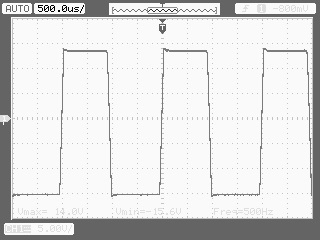
\includegraphics[scale=0.7]{imagens/saturado.jpg} 
\centering
\caption{Sinal de tensão na saída com o cirucito sem o resistor de realimentação.}
\label{fig:saturado} 
\end{figure} 

Observa-se na tabela uma ótima concordância entre os valores obtidos teoricamente com aqueles medidos em laboratório.

\section{Conclusões}

Nesta prática foi estudado o amplificador tipo inversor e não inversor, foi possível realizar sua montagem e fazer a análise do ganho $A_v$ do circuito proposto para diferentes valores resistências de referência. Primeiramente foi analisado o circuito inversor e percebemos que a medida que trocarmos as resistências de referência o sinal de entrada era amplificado e invertido na saída do AMPOP, depois constatou que no circuito não inversor não houve inversão do sinal de entrada na saída. Além disso foi possível notar que quando a resistência de referência é retirada do sistema, o circuito satura, e não amplifica o sinal desejado, não importando o valor sinal de entrada.

\newpage

\section{Anexos}
Vide abaixo as formas de onda obtidas na prática:

\begin{figure}[H] 
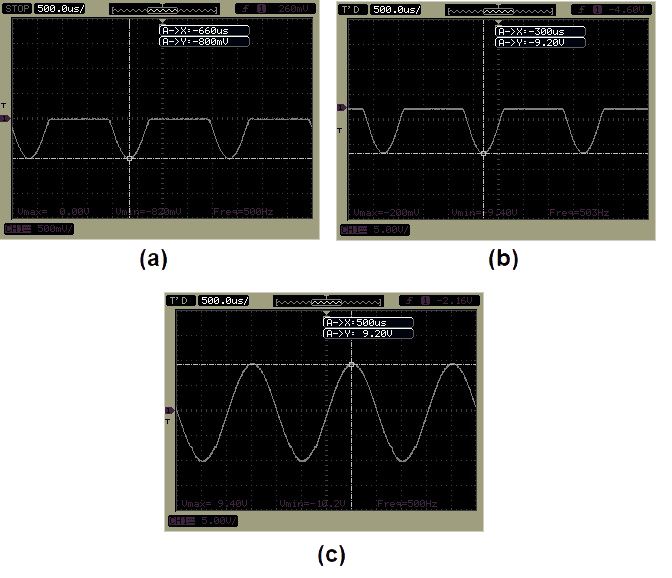
\includegraphics[scale=0.8]{imagens/inv.jpg} 
\centering
\caption{Tensão na saída do circuito inversor para os ganhos de (a) -1, (b) -10 e (c) -100.}
\label{fig:inv} 
\end{figure} 

\begin{figure}[H] 
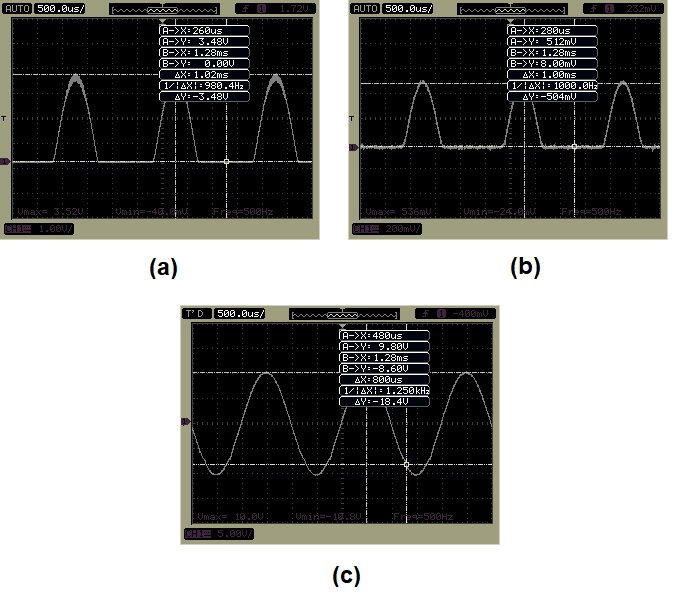
\includegraphics[scale=0.6]{imagens/ninv.jpg} 
\centering
\caption{Tensão na saída do circuito não inversor para os ganhos de (a) 2, (b) 11 e (c) 101.}
\label{fig:ninv} 
\end{figure} 

\begin{figure}[H] 
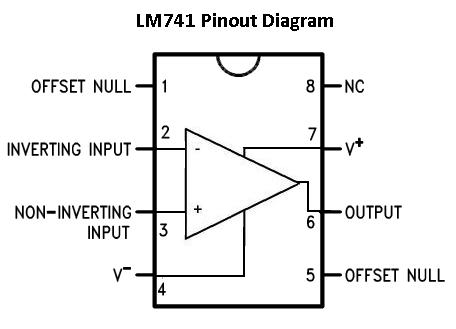
\includegraphics[scale=0.75]{imagens/LM741.jpg} 
\centering
\caption{Pinagem do LM741}
\label{fig:ninv} 
\end{figure} 



Vide em anexo abaixo as folhas de cálculo utilizadas durante o experimento:

\begin{figure}[H] 
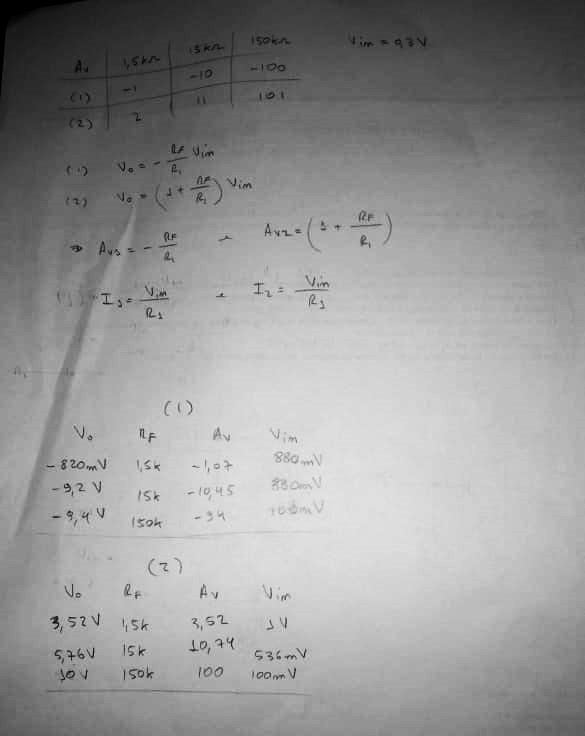
\includegraphics[scale=1]{imagens/calc.png} 
\centering
\caption{Folha de cálculos.}
\label{calc:1} 
\end{figure} 





     






